% =============================================================================
%
% Copyright (c) 2009--2013, Nico Schlömer
% All rights reserved.
%
% Redistribution and use in source and binary forms, with or without
% modification, are permitted provided that the following conditions are
% met:
%
%     * Redistributions of source code must retain the above copyright
%       notice, this list of conditions and the following disclaimer.
%     * Redistributions in binary form must reproduce the above copyright
%       notice, this list of conditions and the following disclaimer in
%       the documentation and/or other materials provided with the distribution
%
% THIS SOFTWARE IS PROVIDED BY THE COPYRIGHT HOLDERS AND CONTRIBUTORS "AS IS"
% AND ANY EXPRESS OR IMPLIED WARRANTIES, INCLUDING, BUT NOT LIMITED TO, THE
% IMPLIED WARRANTIES OF MERCHANTABILITY AND FITNESS FOR A PARTICULAR PURPOSE
% ARE DISCLAIMED. IN NO EVENT SHALL THE COPYRIGHT OWNER OR CONTRIBUTORS BE
% LIABLE FOR ANY DIRECT, INDIRECT, INCIDENTAL, SPECIAL, EXEMPLARY, OR
% CONSEQUENTIAL DAMAGES (INCLUDING, BUT NOT LIMITED TO, PROCUREMENT OF
% SUBSTITUTE GOODS OR SERVICES; LOSS OF USE, DATA, OR PROFITS; OR BUSINESS
% INTERRUPTION) HOWEVER CAUSED AND ON ANY THEORY OF LIABILITY, WHETHER IN
% CONTRACT, STRICT LIABILITY, OR TORT (INCLUDING NEGLIGENCE OR OTHERWISE)
% ARISING IN ANY WAY OUT OF THE USE OF THIS SOFTWARE, EVEN IF ADVISED OF THE
% POSSIBILITY OF SUCH DAMAGE.
%
% =============================================================================
\newpage
\section{Other tips \& tricks}

% \begin{listing}
% \begin{minted}[frame=single,framerule=2pt,color=\color{badred}]{matlab}
% % ===================================================
% % *** FUNCTION simpson
% % ***
% % *** Implements Simpson's rule for integrating
% % *** the sine function over [a,b] with granularity
% % *** h.
% % ***
% % ===================================================
% function int = simpson( a, b, h )
%
%   x = a:h:b;
%
%   int = 0;
%   n   = length(x);
%   mid = (x(1:n-1) + x(2:n)) / 2;
%   int = sum( h/6 * (    sin(x(1:n-1)) ...
%                     + 4*sin(mid     ) ...
%                     +   sin(x(2:n  )) ) );
%
% end
% % ===================================================
% % *** END FUNCTION simpson
% % ===================================================
% \end{minted}
% \caption{Implementation of Simpson's rule for numerically integrating a function (here: \lstinline!sin!) between \lstinline!a! and \lstinline!b!. Note the usage of the vector notation to speed up the function. Also note that \lstinline!sin! is hardcoded into the routine, and needs to be changed each time we want to change the function. In case one is interested in calculating the integral of $f(x) = \exp(\sin(\frac{1}{x})) / \tan(\sqrt{1-x^4})$, this could get quite messy.}
% \label{listing:simpson1}
% \end{listing}


\begin{lstlisting}[
framerule=2pt,
float,
label={listing:simpson1},
caption={Implementation of Simpson's rule for numerically integrating a function (here: \lstinline!sin!) between \lstinline!a! and \lstinline!b!. Note the usage of the vector notation to speed up the function. Also note that \lstinline!sin! is hardcoded into the routine, and needs to be changed each time we want to change the function. In case one is interested in calculating the integral of $f(x) = \exp(\sin(\frac{1}{x})) / \tan(\sqrt{1-x^4})$, this could get quite messy.},
rulecolor=\color{badred}]
% ===================================================
% *** FUNCTION simpson
% ***
% *** Implements Simpson's rule for integrating
% *** the sine function over [a,b] with granularity
% *** h.
% ***
% ===================================================
function int = simpson( a, b, h )

  x = a:h:b;

  int = 0;
  n   = length(x);
  mid = (x(1:n-1) + x(2:n)) / 2;
  int = sum( h/6 * (    sin(x(1:n-1)) ...
                    + 4*sin(mid     ) ...
                    +   sin(x(2:n  )) ) );

end
% ===================================================
% *** END FUNCTION simpson
% ===================================================
\end{lstlisting}

\subsection{Functions as arguments -- \cleansymbol\cleansymbol\cleansymbol}

In numerical computation, there are set-ups which natively treat functions as
the objects of interest, for example when numerically integrating them over a
particular domain. For this example, imagine that you wrote a function that
implements Simpson's integration rule (see listing~\ref{listing:simpson1}),
and you would like to apply it to a number of functions without having to
alter your source code (for example, replacing \lstinline!sin()! by
\lstinline!cos()!, \lstinline!exp()! or something else).

A clean way to deal with this in \matlab{} is using \emph{function handles}. This may sound fancy, and describes nothing else then the capability of treating functions (such as \lstinline!sin()!) as arguments to other functions (such as \lstinline!simpson()!). The function call itself is written as easy as

\begin{lstlisting}[
float,
caption={Simpson's rule with function handles. Note that the syntax for function arguments is no different from that of ordinary ones.},
label={listing:simpson2},
framerule=2pt,
rulecolor=\color{goodgreen}]
% ===================================================
% *** FUNCTION simpson
% ***
% *** Implements Simpson's rule for integrating
% *** a function f over [a,b] with granularity h.
% ***
% ===================================================
function int = simpson( f, a, b, h )

  x   = a:h:b;
  mid = (x(1:n-1) + x(2:n)) / 2;

  n   = length(x);

  int = sum( h/6 * (    f(x(1:n-1)) ...
                    + 4*f(mid     ) ...
                    +   f(x(2:n  )) ) );

end
% ===================================================
% *** END FUNCTION simpson
% ===================================================
\end{lstlisting}

\hfill
\begin{minipage}[t]{.90\textwidth}
\begin{lstlisting}[framerule=1pt,rulecolor=\color{goodgreen}]
a = 0;
b = pi/2;
h = 1e-2;
int_sin = simpson( @sin, a, b, h );
int_cos = simpson( @cos, a, b, h );
int_f   = simpson( @f  , a, b, h );
\end{lstlisting}
\end{minipage}
\hfill

where the function name need to be prepended by the `\lstinline!@!'-character.

The function \lstinline!f()! can be any function that you defined yourself and
which is callable as \lstinline!f(x)! with \lstinline!x! being a vector of $x$
values (like it is used in \lstinline!simpson()!, listing~\ref{listing:simpson2}).



\subsection{Implicit matrix--vector products -- \cleansymbol}

In numerical analysis, almost all methods for solving linear equation systems
\emph{quickly} are iterative methods, that is, methods which define how to
iteratively approach a solution in small steps (starting with some initial
guess) rather then directly solving them in one big step (such as Gau{\ss}ian
elimination). Two of the most prominent iterative methods are CG and GMRES.

In particular, those methods \emph{do not require the explicit availability of
the matrix} as in each step of the iteration they merely form a matrix-vector
product with $A$ (or variations of it). Hence, they technically only need a
function to tell them how to carry out a matrix-vector multiplication. In some
cases, providing such a function may be easier than explicitly constructing
the matrix itself, as the latter usually requires one to pay close attention
to indices (which can get extremely messy).

Beyond that, there may also a mild advantage in memory consumption as the
indices of the matrix do no longer need to sit in memory, but can be hard coded
into the matrix-vector-multiplication function itself. Considering the fact
that we are mostly working with sparse matrices however, this might not be
quite important.

The example below illustrates the typical benefits and drawbacks of the
approach.

\begin{lstlisting}[
float,
framerule=1pt,
caption={Function that implements matrix--vector multiplication with $1/h^2 \times \diag(-1,2,-1)$. Note that the function consumes (almost) no more memory then \lstinline!u! already required.},
label={listing:Amultiply}
]
% ===================================================
% *** FUNCTION A_multiply
% ***
% *** Implements matrix--vector multiplication with
% *** diag[-1,2,-1]/h^2  .
% ***
% ===================================================
function out = A_multiply( u )

  n   = length( u );
  u   = [0; u; 0];

  out = -u(1:n) + 2*u(2:n+1) - u(3:n+2);
  out = out * (n+1)^2;

end
% ===================================================
% *** END FUNCTION A_multiply
% ===================================================
\end{lstlisting}


\hfill
\begin{minipage}[t]{.45\textwidth}
\begin{lstlisting}[framerule=1pt]
n = 1e3;
k = 500;







u = ones(n,1);
for i=1:k
    u = A_multiply( u );
end
\end{lstlisting}
Computing $u = A^ku_0$ with the function \lstinline!A_multiply!
(listing~\ref{listing:Amultiply}). The memory consumption of this routine is
(almost) no greater than storing $n$ real numbers. Execution time:
\extime{21}.
\end{minipage}
\hfill
\begin{minipage}[t]{.45\textwidth}
\begin{lstlisting}[framerule=1pt]
n = 1e3;
k = 500;

e = ones(n,1);
A = spdiags([-e,2*e,-e],...
            [-1,  0,-1],...
             n, n );
A = A * (n+1)^2;

u = ones(n,1);
for i=1:k
    u = A*u;
end
\end{lstlisting}
Computing $u = A^ku_0$ with a regular sparse format matrix \lstinline!A!, with the need to store it in memory. Execution time: \extime{7}.
\end{minipage}
\hfill

All in all, these considerations shall not lead you to rewrite all you
matrix-vector multiplications as function calls. Mind, however, that there are
situations where one would \emph{never} use matrices in their explicit form,
although mathematically written down like that:

\begin{example}[Multigrid]
In geometric multigrid methods, a domain is discretized with a certain
parameter $h$ (``grid width'') and the operator $A_h$ written down for that
discretization (see the examples above, where $A_h=h^{-2}\diag(-1,2,1)$ is
really the discretization of the $\Delta$-operator in one dimension). In a
second step, another, somewhat coarser grid is considered with $H=2h$, for
example. The operator $A_H$ on the coarser grid is written down as
\[
A_H = I_h^H A_h I_H^h,
\]
where the $I_*^*$ operators define the transition from the coarse to the fine
grid, or the other way around. When applying it to a vector on the coarse grid
$u_H$ ($A_Hu_H =I_h^H A_h I_H^h u_H$), the above definition reads:
\begin{enumerate}
\item $I_H^h u_H$: Map $u_H$ to the fine grid.
\item $A_h\cdot$: Apply the fine grid operator to the transformation.
\item $I_h^H\cdot$: Transform the result back to the coarse grid.
\end{enumerate}
How the transformations are executed needs to be defined. One could, for
example, demand that $I_H^h$ maps all points that are part of the fine grid
\emph{and} the coarse grid to itself; all points on the fine grid, that lie
right in between two coarse variables get half of the value of each of the two
(see figure~\ref{subfig:coarse-fine}).

\begin{figure}
\centering
\begin{subfigure}{0.45\textwidth}
  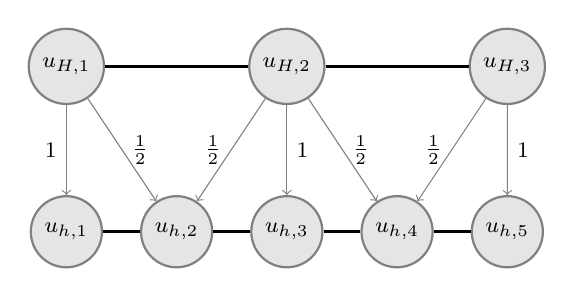
\begin{tikzpicture}[node/.style={circle,draw=black!50,fill=black!10,thick,font=\footnotesize},scale=0.7,
arrownote/.style={black,font=\footnotesize}]


\node (u1) at (0,3) [node] {$u_{H,1}$};
\node (u2) at (4,3) [node] {$u_{H,2}$};
\node (u3) at (8,3) [node] {$u_{H,3}$};


\node (u5) at (0,0) [node] {$u_{h,1}$};
\node (u6) at (2,0) [node] {$u_{h,2}$};
\node (u7) at (4,0) [node] {$u_{h,3}$};
\node (u8) at (6,0) [node] {$u_{h,4}$};
\node (u9) at (8,0) [node] {$u_{h,5}$};

\draw [very thick] (u1) -- (u2) --(u3);
\draw [very thick] (u5) --(u6) --(u7) --(u8) --(u9);

\draw [->,black!50] (u1) to node [arrownote,left] {$1$}  (u5) ;
\draw [->,black!50] (u1) to node [arrownote,right] {$\frac{1}{2}$} (u6) ;

\draw [->,black!50] (u2) to node [arrownote,left] {$\frac{1}{2}$} (u6) ;
\draw [->,black!50] (u2) to node [arrownote,right] {$1$} (u7) ;
\draw [->,black!50] (u2) to node [arrownote,right] {$\frac{1}{2}$} (u8) ;

\draw [->,black!50] (u3) to node [arrownote,left] {$\frac{1}{2}$} (u8) ;
\draw [->,black!50] (u3) to node [arrownote,right] {$1$} (u9) ;

\end{tikzpicture}
  \caption{Possible transformation rule when translating values from the
  coarse to the fine grid. See listing~\ref{listing:IHh}.}
  \label{subfig:coarse-fine}
\end{subfigure}
\hfill
\begin{subfigure}{0.45\textwidth}
  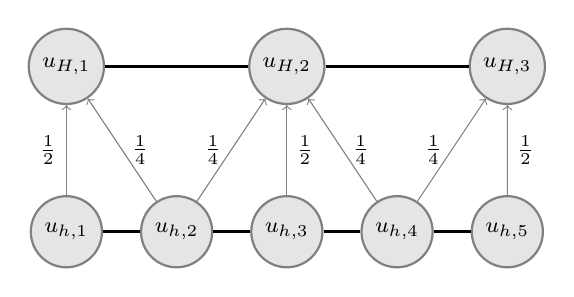
\begin{tikzpicture}[
node/.style={circle,draw=black!50,fill=black!10,thick,font=\footnotesize},scale=0.7,
arrownote/.style={black,font=\footnotesize}]

\node (u1) at (0,3) [node] {$u_{H,1}$};
\node (u2) at (4,3) [node] {$u_{H,2}$};
\node (u3) at (8,3) [node] {$u_{H,3}$};

\node (u5) at (0,0) [node] {$u_{h,1}$};
\node (u6) at (2,0) [node] {$u_{h,2}$};
\node (u7) at (4,0) [node] {$u_{h,3}$};
\node (u8) at (6,0) [node] {$u_{h,4}$};
\node (u9) at (8,0) [node] {$u_{h,5}$};

\draw [very thick] (u1) -- (u2) --(u3);blue
\draw [very thick] (u5) --(u6) --(u7) --(u8) --(u9);

\draw [->,black!50] (u5) to node [arrownote,left] {$\frac{1}{2}$}  (u1) ;
\draw [->,black!50] (u6) to node [arrownote,right] {$\frac{1}{4}$} (u1) ;

\draw [->,black!50] (u6) to node [arrownote,left] {$\frac{1}{4}$} (u2) ;
\draw [->,black!50] (u7) to node [arrownote,right] {$\frac{1}{2}$} (u2) ;
\draw [->,black!50] (u8) to node [arrownote,right] {$\frac{1}{4}$} (u2) ;

\draw [->,black!50] (u8) to node [arrownote,left] {$\frac{1}{4}$} (u3) ;
\draw [->,black!50] (u9) to node [arrownote,right] {$\frac{1}{2}$} (u3) ;

\end{tikzpicture}

  \caption{Mapping back from fine to coarse.}
  \label{subfig:fine-coarse}
\end{subfigure}
\caption{}
\end{figure}


\begin{lstlisting}[
float,
framerule=1pt,
caption={Function that implements the operator $I_H^h$ from the example (see figure~\ref{subfig:coarse-fine}). Writing down the structure of the corresponding matrix would be somewhat complicated, and even more so when moving to two- or three-dimensional grids. Note also how matrix notation has been exploited.},
label={listing:IHh}
]
% ===========================================================
% *** FUNCTION coarse2fine
% ***
% *** Transforms values from a coarse grid to a fine grid.
% ***
% ===========================================================
function uFine = coarse2fine( uCoarse )

  N = length(uCoarse);
  n = 2*N - 1;

  uFine(1:2:n) = uCoarse;

  midValues    = 0.5 * ( uCoarse(1:N-1) + uCoarse(2:N) );
  uFine(2:2:n) = midValues;

end
% ===========================================================
% *** END FUNCTION coarse2fine
% ===========================================================
\end{lstlisting}


In the analysis of the method, $I_H^h$ and $I_h^H$ will always be treated as
matrices, but when implementing, one would \emph{certainly not} try to figure
out the structure of the matrix. It is a lot simpler to implement a function
that executes the rule suggested above, for example.
\end{example}
